% Mirror: https://github.com/SIGma-UIUC/presentation-format
% --------------------------------------------------------------------
% This is a simple Beamer document that uses beamerthemesigma.sty
% Reading the comments should help you create a presentation even if
% you've never used Beamer before.
% --------------------------------------------------------------------

% Set our document class to Beamer
\documentclass[aspectratio=169]{beamer}
% \documentclass[aspectratio=169, handout]{beamer}
% Add handout option to ignore pauses

% From Jeff E
\usepackage{algo}
% Some more macros
\usepackage{sigmastyle}


% Set a title
\title{What are Codes?}

% Set a subtitle if you desire
\subtitle{\cite{good_vid}}

% Whoever worked on the presentation:
\author{Anakin}

% Date looks ugly, so leave blank
\date{}

% An institute name, if you're so inclined
% \institute{University of Illinois Urbana-Champaign}

% Use the SIGma theme for this Beamer presentation
\usetheme{sigma}
% --------------------------------------------------------------------

% Begin document
\begin{document}

% Beamer calls each slide a "frame", defined within the environment:
% \begin{frame}
%   <frame content here>
% \end{frame}

% This frame is just the title.
\begin{frame}
\titlepage
\end{frame}

\begin{frame}{Updates!}
  % Let's put some real content in this frame:
  Weekly updates:
  \begin{itemize}
    \item I will be presenting more of my REU work \textcolor{sigma@mainblue}{this Friday}!
    \item Everitt Hall Room 2233 at 4PM!
    \item THERE IS FREE PIZZA!!
  \end{itemize}
\end{frame}

\section{Motivation}
\frame{\sectionpage}

\begin{frame}{The Basic Problem}
    Let $x[1\ldots k]$ be some (bit)string\pause
    \[
        x[1\ldots k] \xrightarrow[]{\textsc{encode}(x)} c[1 \ldots n] \pause \xrightarrow[]{\textcolor{sigma@alertred}{\textsc{corruption}}} \tilde{c}[1 \ldots n]
    \]\pause
    \begin{center}
        \textcolor{sigma@mainblue}{\textbf{Question:}} Can we design \textsc{encode} such that we can recover $x$ from $\tilde{c}$?
    \end{center}
\end{frame}

\begin{frame}{In Space No One Can Hear You \st{Scream} Bitflip}
    Here's one of the most entertaining reasons why we care about this problem
    \begin{itemize}
        \item A 2003 national election in Belgium used electronic voting \pause
        \item A little known candidate got more votes than were people in the town that reported an error \pause
        \item A recount was done and the candidates votes decreased by $4096 = 2^{12}$ \pause
        \item An investigation later determined that the a bit in the magnetic cards being used got flipped due to a cosmic ray (after ruling out other causes)
    \end{itemize}
\end{frame}

\section{Making This Concrete}
\frame{\sectionpage}

\begin{frame}{ABCs of Codes}
    \begin{defn}[Alphabets, Block Lengths, Codes]
        A \emph{code} $C$ of \emph{block length} $n$ over a (finite) alphabet $\Sigma$ is a set $C \subseteq \Sigma^n$.
        
        An element $c \in C$ is a \emph{code word} (big surprise here).
    \end{defn} 
\end{frame}

\begin{frame}{An Example}
    Consider the following encoding over $\Sigma = \set{0, 1}$ (bitstrings)
    \begin{align*}
        \textsc{encode}\colon \set{0, 1}^3 &\to \set{0, 1}^4 \\
                    (x_1, x_2, x_3) &\mapsto (x_1, x_2, x_3, x_1 + x_2 + x_3 \pmod{2})
    \end{align*} \pause
    \[
        C \defeq \im(\textsc{encode}) = \begin{Bmatrix}
                0000, & 0011, & 0101, & 0110 \\
                1001, & 1010, & 1100, & 1111
        \end{Bmatrix}
    \] \pause
    \textcolor{sigma@mainblue}{\textbf{Claim:}} Code $C$ can \ul{correct} one erasure.
    If we lose one bit and know where it was, we can recover it.\pause

    If $\tilde{c} =  0{\color{sigma@alertred}?}01$, what is $c$? \pause {\color{sigma@mainblue} $c = 0101$} \pause
    
    If $\tilde{c} =  11{\color{sigma@alertred}?}1$, what is $c$? \pause {\color{sigma@mainblue} $c = 1111$} \pause
    
    If $\tilde{c} =  0{\color{sigma@alertred}??}1$, what is $c$? \pause {\color{sigma@alertred} $c = 0101$ or $c = 0011$}
\end{frame}

\begin{frame}{An Example}
    Consider the following encoding over $\Sigma = \set{0, 1}$ (bitstrings)
    \begin{align*}
        \textsc{encode}\colon \set{0, 1}^3 &\to \set{0, 1}^4 \\
                    (x_1, x_2, x_3) &\mapsto (x_1, x_2, x_3, x_1 + x_2 + x_3 \pmod{2})
    \end{align*}
    \[
        C \defeq \im(\textsc{encode}) = \begin{Bmatrix}
                (0, 0, 0, 0), & (0, 0, 1, 1), & (0, 1, 0, 1), & (0, 1, 1, 0), \\
                (1, 0, 0, 1), & (1, 0, 1, 0), & (1, 1, 0, 0), & (1, 1, 1, 1)
            \end{Bmatrix}
    \]
    \textcolor{sigma@mainblue}{\textbf{Claim:}} Code $C$ can \ul{detect} one error. 
    We can tell detect with certainty if $\tilde{c} \in C$ or $\tilde{c} \notin C$ if at most one bit was flipped \pause

    If $\tilde{c} =  0001$, was there an error? \pause \textcolor{sigma@mainblue}{YES!} what is $c$? \pause $c \in \set{0000, 1001, 0101, 0011}$ \pause
    
    If $\tilde{c} =  0000$, was there an error? \pause \textcolor{sigma@mainblue}{Who knows?} $c$ could be $0000$ or $0110$
\end{frame}

\begin{frame}{Metrics and Geometry}
        Consider the following encoding over $\Sigma = \set{0, 1}$ and  $C \defeq \im(\textsc{encode})$
    \begin{align*}
        \textsc{encode}\colon \set{0, 1}^4 &\to \set{0, 1}^7 \\
                    (x_1, x_2, x_3, x_4) &\mapsto (x_1, x_2, x_3, x_4, \overbrace{x_2 + x_3 + x_4, x_1 + x_3 + x_4, x_1 + x_2 + x_4}^{\text{mod }2})
    \end{align*}

    \textcolor{sigma@mainblue}{\textbf{Claim:}} This code can \ul{correct} one error! 
    So we can tell if $\tilde{c} \in C$ or if $\tilde{c} \notin C$ and there is one flipped bit, we can correct it. \pause

    We will show this geometrically
\end{frame}

\begin{frame}{}
\[
(x_1, x_2, x_3, x_4) \mapsto (x_1, x_2, x_3, x_4, \overbrace{x_2 + x_3 + x_4, x_1 + x_3 + x_4, x_1 + x_2 + x_4}^{\text{mod }2})
\]
\textcolor{sigma@alertred}{\textbf{Question:}} If $\tilde{c} = 0111010$, what is $c$? \pause
    \includegraphics[width=\textwidth]{images/coding-01.png}
\end{frame}

\begin{frame}{}
\[
(x_1, x_2, x_3, x_4) \mapsto (x_1, x_2, x_3, x_4, \overbrace{x_2 + x_3 + x_4, x_1 + x_3 + x_4, x_1 + x_2 + x_4}^{\text{mod }2})
\]
\textcolor{sigma@alertred}{\textbf{Question:}} If $\tilde{c} = 0111010$, what is $c$?
    \includegraphics[width=\textwidth]{images/coding-02.png}
\end{frame}
\begin{frame}{}
\[
(x_1, x_2, x_3, x_4) \mapsto (x_1, x_2, x_3, x_4, \overbrace{x_2 + x_3 + x_4, x_1 + x_3 + x_4, x_1 + x_2 + x_4}^{\text{mod }2})
\]
\textcolor{sigma@alertred}{\textbf{Question:}} If $\tilde{c} = 0111010$, what is $c$?
    \includegraphics[width=\textwidth]{images/coding-03.png}
\end{frame}
\begin{frame}{}
\[
(x_1, x_2, x_3, x_4) \mapsto (x_1, x_2, x_3, x_4, \overbrace{x_2 + x_3 + x_4, x_1 + x_3 + x_4, x_1 + x_2 + x_4}^{\text{mod }2})
\]
\textcolor{sigma@alertred}{\textbf{Question:}} If $\tilde{c} = 0111010$, what is $c$?
    \includegraphics[width=\textwidth]{images/coding-04.png}
\end{frame}
\begin{frame}{}
\[
(x_1, x_2, x_3, x_4) \mapsto (x_1, x_2, x_3, x_4, \overbrace{x_2 + x_3 + x_4, x_1 + x_3 + x_4, x_1 + x_2 + x_4}^{\text{mod }2})
\]
\textcolor{sigma@alertred}{\textbf{Question:}} If $\tilde{c} = 0111010$, what is $c$? \hfill \textcolor{sigma@mainblue}{\textbf{Answer:}} $c = 0101010$
    \includegraphics[width=\textwidth]{images/coding-05.png}
\end{frame}

\begin{frame}{Formalizing What We Just Saw}
    The code we just saw is an example of the \emph{Hamming Code}.
    \begin{defn}[(Relative) Hamming Distance]
        The \emph{Hamming Distance} $\Delta(x, y)$ between $x, y \in \Sigma^n$ is the number of positions where $x$ and $y$ have different characters. \pause
        
        \textcolor{sigma@alertred}{\textbf{Exercise:}} If you know what a metric is, this is a metric. $\forall x, y, z \in \Sigma^n$:
        \begin{itemize}
            \item $\Delta(x, x) = 0$, $\Delta(x, y) = \Delta(y, x)$, If $x \neq y$, $\Delta(x, y) > 0$
            \item $\Delta(x, z) \leq \Delta(x, y) + \Delta(y, z)$ (Triangle Inequality)
        \end{itemize}
        \pause
    
        The \emph{Relative Hamming Distance} $\delta(x, y)$ is $\frac{\Delta(x, y)}{n}$.
    \end{defn} \pause

    \begin{defn}[Minimum Distance]
        The \emph{Minimum Distance} of a code $C$ is $\Min_{x \neq y \in C} \Delta(x, y)$
    \end{defn}
\end{frame}

\begin{frame}{Robustness of a Code}
    \begin{thrm}
        A code with minimum distance $d$ can
        \begin{enumerate}
            \item Correct $\leq d - 1$ erasures
            \item Detect $\leq d - 1$ errors
            \item Correct $\floor{\frac{d - 1}{2}}$ errors
        \end{enumerate}
    \end{thrm} \pause
    
    \textcolor{sigma@mainblue}{Examples:} (Go check these!)
    \begin{itemize}
        \item The first code we saw $\textsc{encode}\colon \Sigma^3 \to \Sigma^4$ has distance $2$
        \item The second code we saw $\textsc{encode}\colon \Sigma^4 \to \Sigma^7$ has distance $3$
    \end{itemize} \pause

    \textcolor{sigma@mainblue}{\textbf{Proof}:} Pretty Pictures
\end{frame}

\begin{frame}{}
    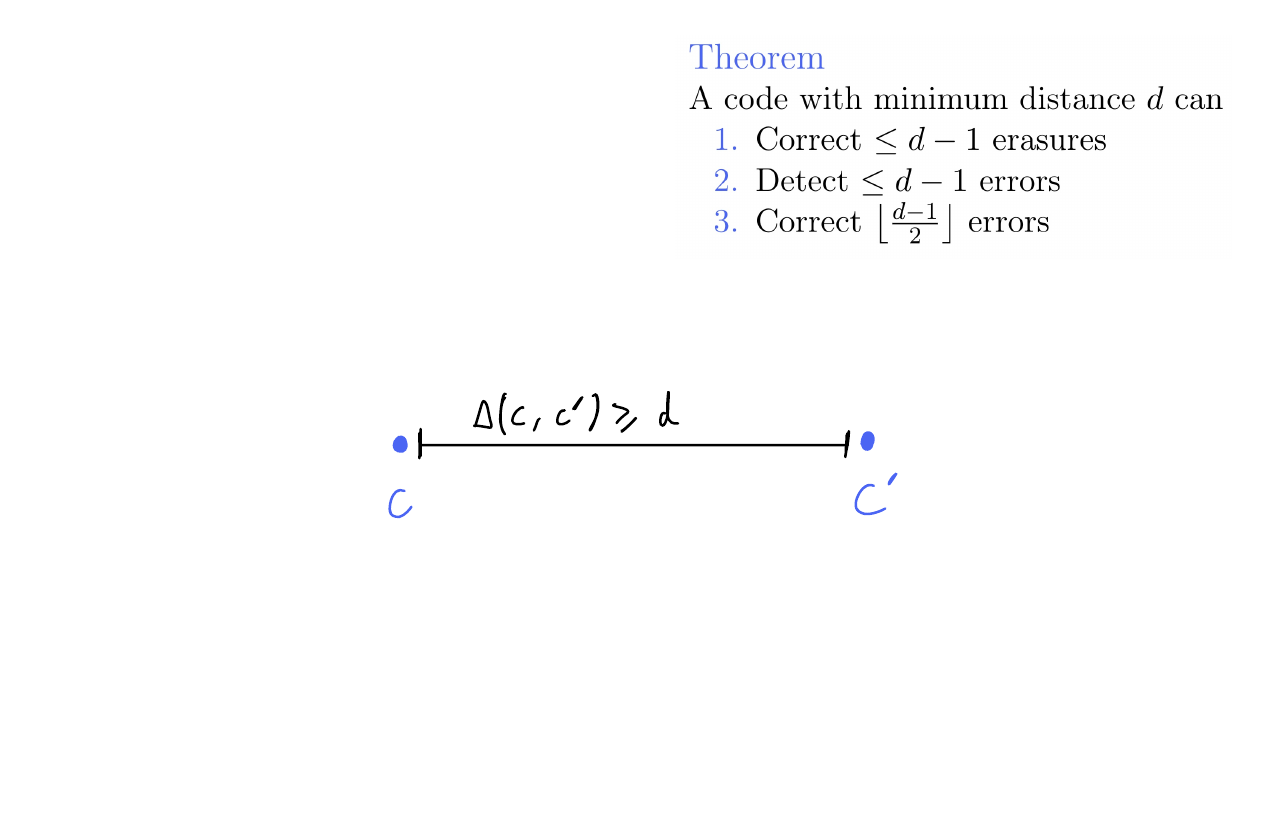
\includegraphics[width=\textwidth]{images/coding-06.png}
\end{frame}
\begin{frame}{}
    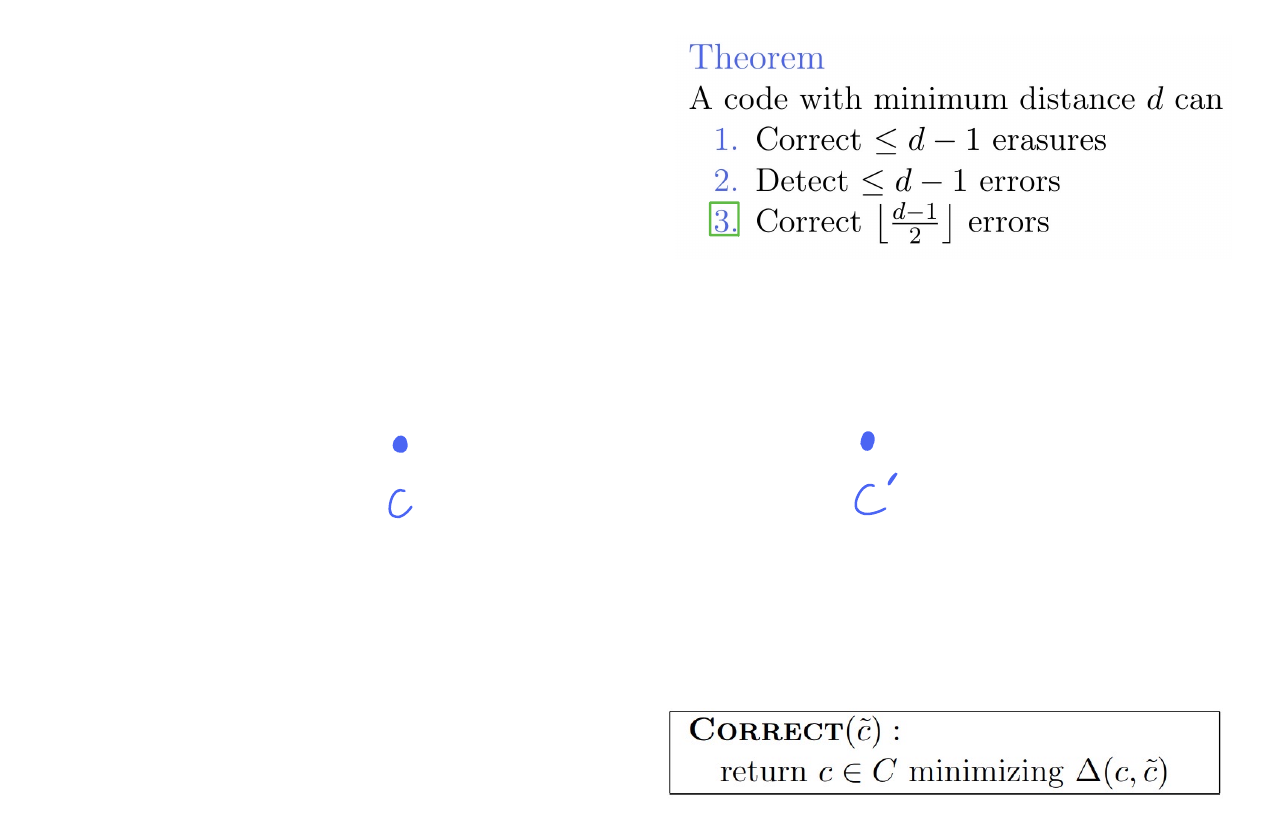
\includegraphics[width=\textwidth]{images/coding-07.png}
\end{frame}
\begin{frame}{}
    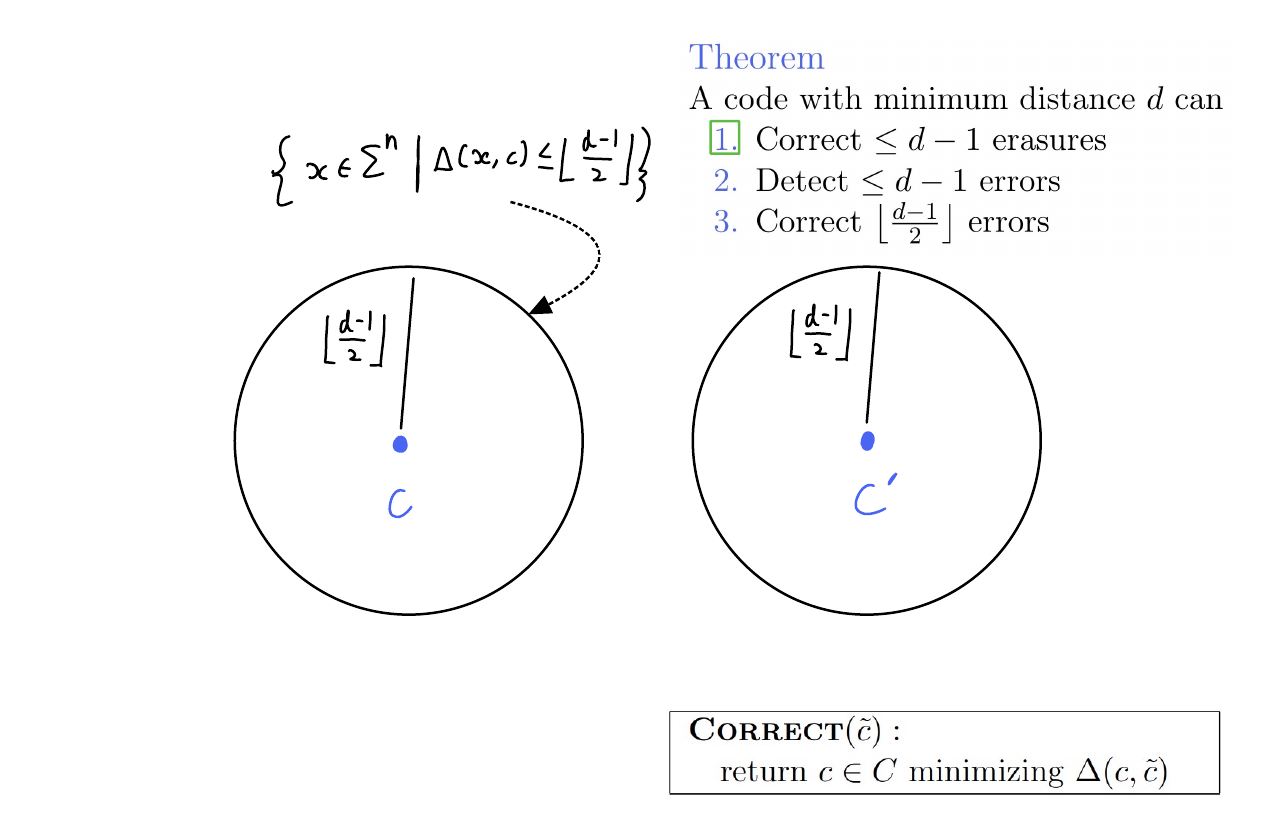
\includegraphics[width=\textwidth]{images/coding-08.png}
\end{frame}
\begin{frame}{}
    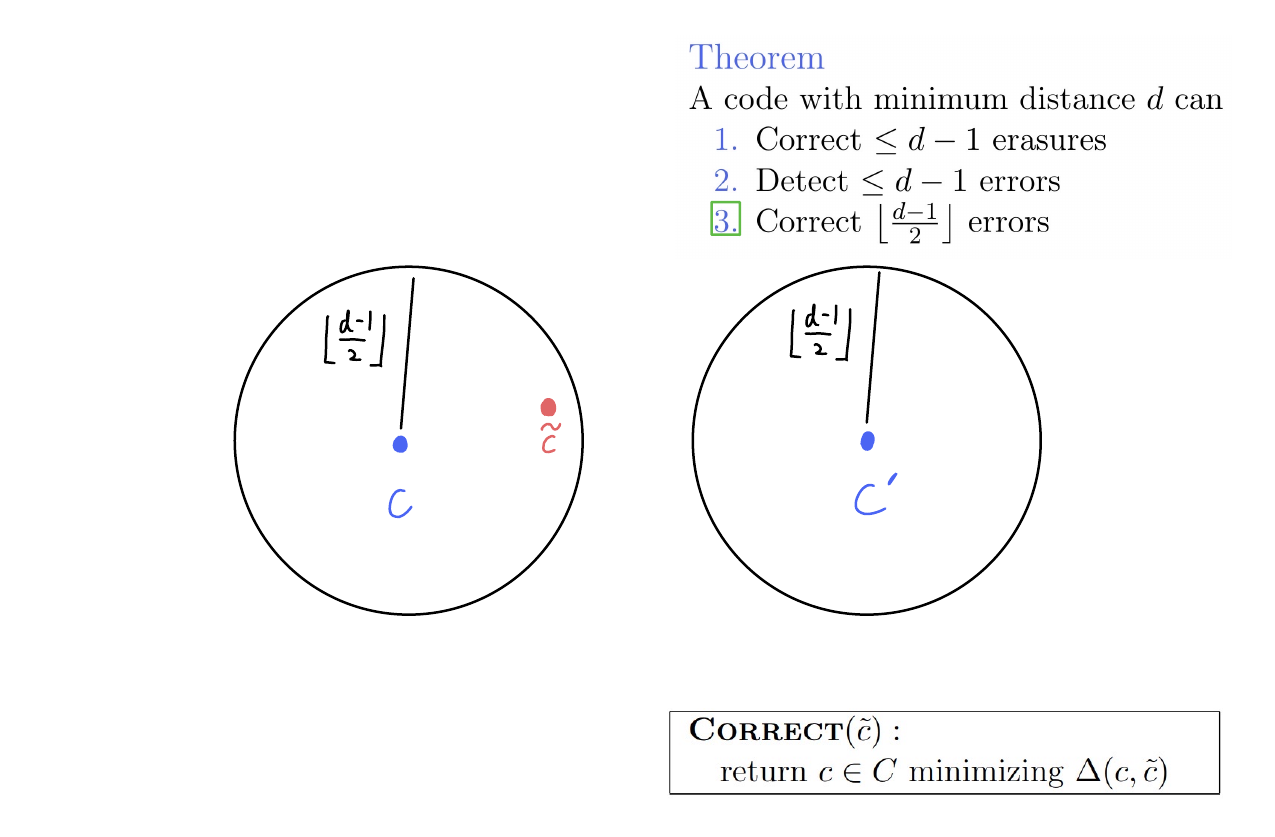
\includegraphics[width=\textwidth]{images/coding-09.png}
\end{frame}
\begin{frame}{}
    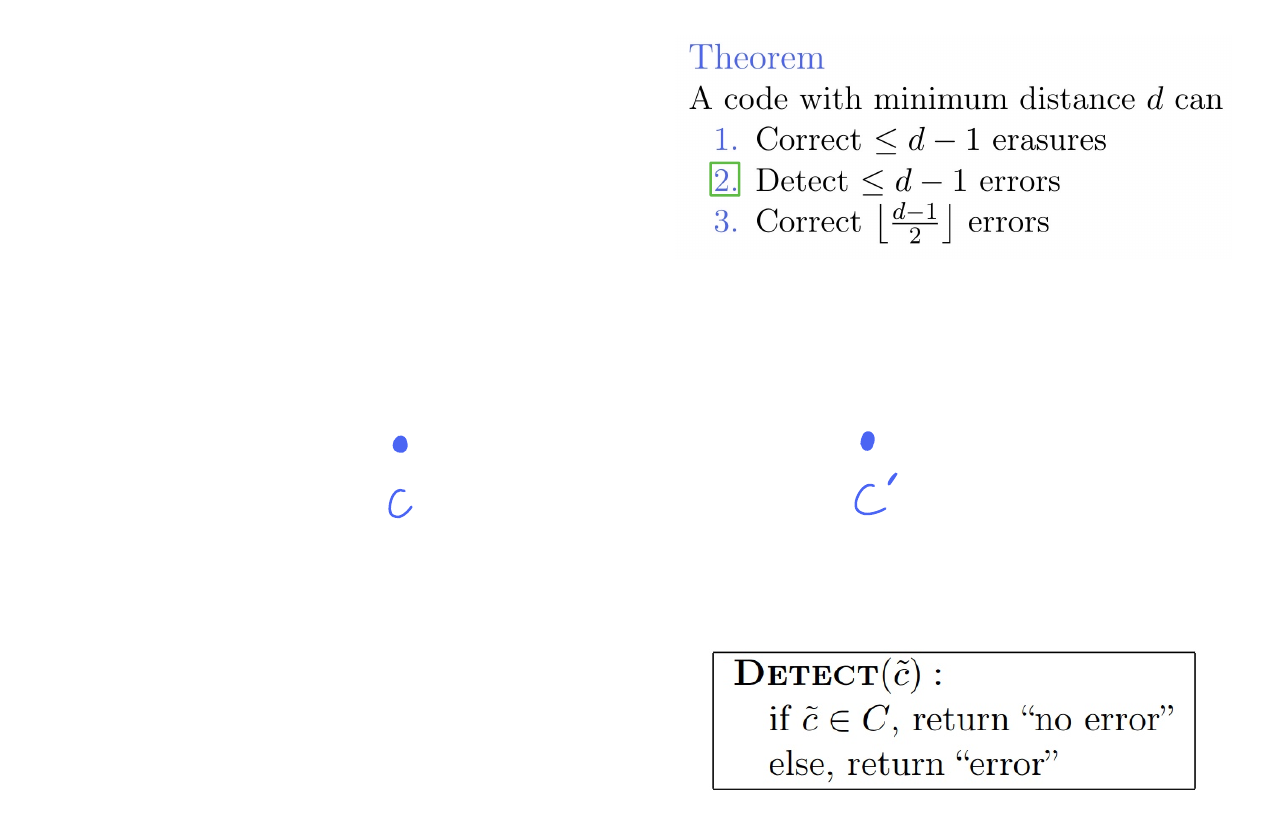
\includegraphics[width=\textwidth]{images/coding-10.png}
\end{frame}
\begin{frame}{}
    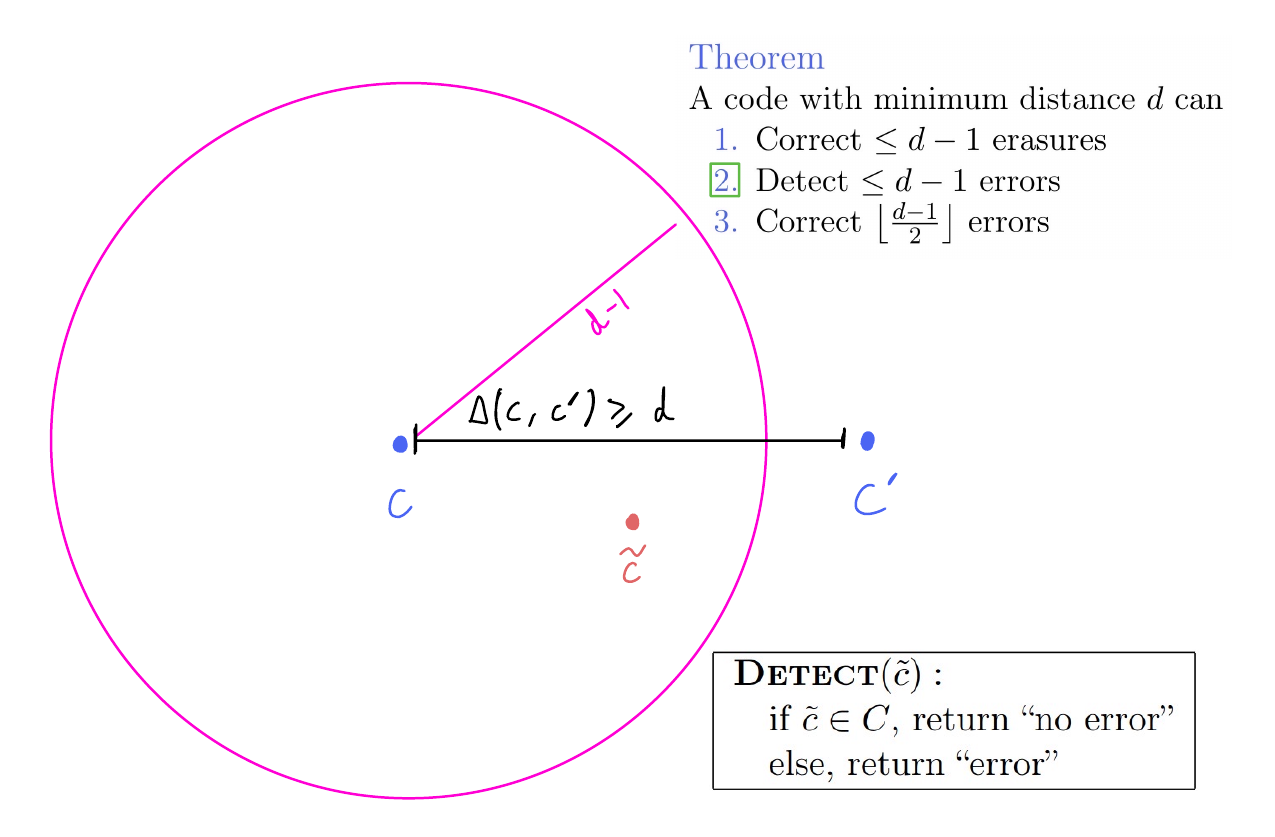
\includegraphics[width=\textwidth]{images/coding-11.png}
\end{frame}

\begin{frame}{}
    What is an erasure?
    \begin{align*}
        c &=         &x_1 && x_2 && x_3 && x_4 && x_5 && x_6 && x_7 && x_8\cdots \\
        \tilde{c} &= &x_1 && x_2 && \_  && \_  && x_5 && \_  && x_7 && x_8\cdots \\
    \end{align*}
    \textcolor{sigma@alertred}{\textbf{Question:}} If there are $\leq d - 1$ erasures, what is the max value of $\Delta(c, \tilde{c})$? \pause

    \textcolor{sigma@mainblue}{\textbf{Answer:}} $d - 1$!
\end{frame}

\begin{frame}{}
    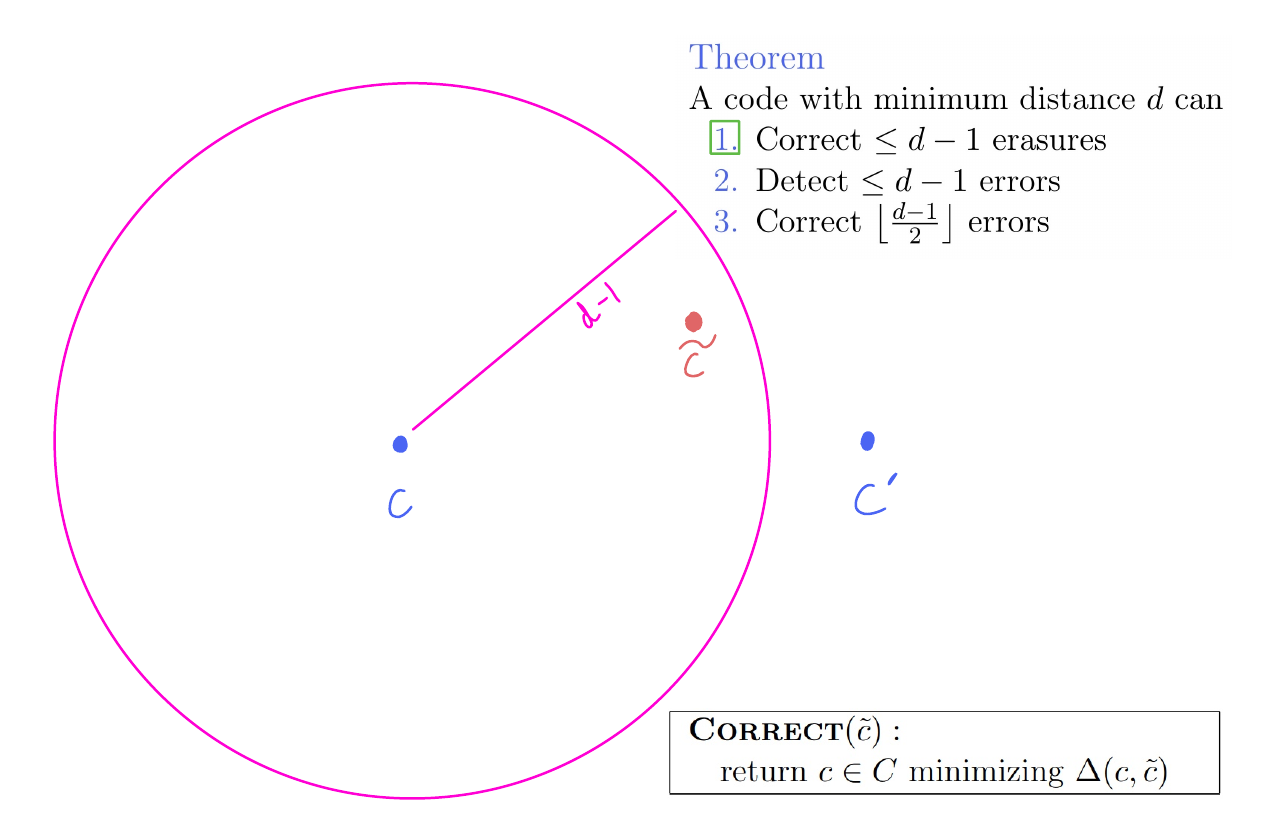
\includegraphics[width=\textwidth]{images/coding-12.png}
\end{frame}

\begin{frame}{Sadly, Pictures are Misleading}
    You may ask ``If $\tilde{c}$ is of distance $\leq d - 1$ to $c$ and $c'$ can be as close as $c'$ then could $\tilde{c}$ be closer to $c'$?''
    \begin{itemize}
        \item Suppose that $\tilde{c}$ is a corruption of $c$ and has $\leq d - 1$ erasures. 
        Suppose $c'$ is a different code word to $c$ but for contradiction, $\Delta(\tilde{c}, c') < \Delta(\tilde{c}, c)$ so $\textbf{\textsc{Correct}}(\tilde{c})$ incorrectly corrects $\tilde{c}$ to $c'$ \pause
        \item That means there are two different ways to fill the $\leq d - 1$ erasures where one filling gives $c$ and the other gives $c'$  \pause
        \item Since we are only dealing with erasures in $\leq d - 1$, we know what the other characters are, and the other $n - d + 1$ positions of $c'$ and $c$ must match.
        \item This implies $\Delta(c, c') \leq d - 1 < d$ which is a contradiction to our minimum distance $d$, since $c$ and $c'$ are distinct strings. 
        So $\textbf{\textsc{Correct}}(\tilde{c})$ should correctly return $c$ 
    \end{itemize}
\end{frame}


\begin{frame}{Efficiency and Overhead}
    \begin{defn}[Message Length]
        The \emph{message length / dimension} of a code $C$ over an alphabet $\Sigma$ is $k \defeq \log_\abs{\Sigma} \abs{C}$
    \end{defn}

    Remember we were talking at the beginning of encoding messages of length $k$ into a code $C$ of messages of length $n$?
    This is the same $k$?

    \begin{itemize}
        \item Our messages live in $\Sigma^k$ and get mapped to a code in $C$ \pause
        \item We want every code word in $C$ to correspond to exactly one message and every message to map to exactly one code word
        \begin{itemize}
            \item Want $\abs{C} = \abs{\Sigma^k} = \abs{\Sigma^k}$
        \end{itemize} \pause
        \item Rearranging yields $k = \log_\abs{\Sigma} \abs{C}$
    \end{itemize}
\end{frame}

\begin{frame}{Efficiency and Overhead}
    \begin{defn}[Rate]
        The \emph{rate} of a code $C \subseteq \Sigma^n$ is $R = \frac{\text{message length }k}{\text{block length }n} = \frac{\log_\abs{\Sigma}\abs{C}}{n}$
    \end{defn}\pause
    \begin{itemize}
        \item $R \in [0, 1]$
        \item This is sort of the measure of the efficiency of the code \pause
        \item $R$ close to 1 means message does not grow that much after encoding
        \item $R$ close to 0 means messages grows quite alot
    \end{itemize}
\end{frame}

\begin{frame}{Trade-offs}
    Consider an encoding $x \mapsto c$ which perhaps gets corrupted into $\tilde{c}$
    \begin{itemize}
        \item We want to handle when something bad happens to $c$
        \item We want to recover information about $x$ from $c / \tilde{c}$ 
    \end{itemize}
\end{frame}

\begin{frame}{Trade-offs}
    Consider an encoding $x \mapsto c$ which perhaps gets corrupted into $\tilde{c}$
    \begin{itemize}
        \item We want \textcolor{sigma@mainblue}{distance $d$} \pause
        \item We want to minimize overhead
    \end{itemize}
\end{frame}

\begin{frame}{Trade-offs}
    Consider an encoding $x \mapsto c$ which perhaps gets corrupted into $\tilde{c}$
    \begin{itemize}
        \item We want \textcolor{sigma@mainblue}{distance $d$} 
        \item We want \textcolor{sigma@mainblue}{rate as close to $1$ as possible}
    \end{itemize}

    \textcolor{sigma@mainblue}{\textbf{Motivating Question:}} What is the trade-off between distance and rate? 
\end{frame}

% Asking questions is fun but we should answer some first
\begin{frame}{}
      \begin{center}
    {\color{sigma@mainblue} \LARGE Questions?}
  \end{center}
\end{frame}

% Quotes are fun, find some to use!
\font\eightss=cmssq8
\font\eightssi=cmssqi8
\newcommand\quoteAuthorDate[3]{\begingroup
  \baselineskip 10pt
  \parfillskip 0pt
  \interlinepenalty 10000 % not needed in example
  \leftskip 0pt plus 40pc minus \parindent
  \let\rm=\eightss
  \let\sl=\eightssi
  \everypar{\sl}#1\par
  \nobreak\smallskip
  \noindent\rm--- #2\unskip\enspace(#3)\par
  \endgroup}
% If someone can figure out how to horizontally center this and make the text bigger that'd be cool
\begin{frame}
    \begin{center}
        \item \quoteAuthorDate{Information is the resolution of uncertainty.}{CLAUDE E SHANNON}{\color{sigma@mainblue} 1948}
    \end{center}
\end{frame}

% Remove this slide if you came up with all the material yourself
\begin{frame}{Bibliography}
    \bibliography{refs}
    \bibliographystyle{alpha}
\end{frame}

\end{document}